\chapter{Вглубь атома}

\epigraph{\emph{... принципиальный вопрос, почему в материальном мире мы снова и снова встречаем повторяющиеся формы и качества}}
{Вернер Гейзенберг}

В книгах по математическим вопросам ядерной физики зачастую принято без долгих предисловий переходить к математическим моделям из сложных уравнений и длинных формул.
При этом изложение обычно ведется на принятом в математике высоком уровне строгости.
Это имеет свой смысл.
Дело в том, что оформившаяся математическая теория того или иного физического процесса вполне может быть изложена отдельно от своего физического контекста.
К сожалению, такого рода книги обычно носят довольно академический характер и понятны только узкому кругу специалистов, имеющих должный уровень математической подготовки. Для первого погружения в задачу, такой подход подходит плохо.

Математику, стоящую за современной ядерной физикой, не стоит на начальном этапе пытаться рассматривать в отрыве от самого ее предмета - атома.
Для полного понимания используемых математических моделей крайне полезно хотя бы в общих чертах понимать как физику атома, так и полные проб и ошибок пути, которые привели ученых к их ключевым идеям.
  
На протяжении всей книги нам не потребуются ни глубокие факты современной ядерной физики, ни продвинутый аппарат квантовой механики.
Вполне достаточно будет общих фактов о строении атома и ядерных реакциях, без которых было бы крайне тяжело понять, почему те или иные задачи ставились перед физиками и математиками Манхэттенского проекта.

В данной главе мы в общих чертах проследим весь путь самой идеи об атоме от туманных философских догадок в древности вплоть до современной точки зрения. 
У нас нет цели глубоко погружаться в историко-философские вопросы атомизма.
Мы наметим лишь общий ход его истории как мировоззрения, останавливаясь только на наиболее ярких идеях и открытиях древних и современных ученых.
В конце главы мы опишем модель атома и процесса ядерного распада, принятые сегодня и не слишком отличающиеся от известных во времена Манхэттенского проекта.
Читатель, знакомый с основами физики атома, может пропустить эту главу и сразу перейти к математической сути вопроса в гл.~\ref{why_math}.

\section*{Первые идеи}

С древнейших времен не прекращались попытки человека проникнуть в суть материальных объектов, мысленно разбив их на минимально возможные части.
Вообще говоря, это универсальный метод исследования любых сложных объектов - пытаться разложить их на более простые, желательно элементарные части. 
Далее следует следует изучить отдельно каждую часть и то, как они взаимодействуют друг с другом.
Поэтому не столь удивительно, что ученые древности пытались найти и описать первоэлементы, из которых должны состоять все объекты окружающего мира.
История этих попыток насчитывает более двух с половиной тысяч лет.

Начало истории об атоме теряется в древних веках.
Доподлинно неизвестно, когда и кому впервые пришла в голову знаменательная идея о том, что все наблюдаемые в природе объекты при всем многообразии их форм и свойств обязаны состоять из небольшого числа \textit{элементарных}.
Наиболее хорошо восстановлен и изучен античный атомизм, но и греки переняли его от более древних цивилизаций Востока, Вавилона и, вероятно, Египта.
Важно, что именно в древней Греции атомизм заиграли всеми красками, глубоко проникая и давая плоды в философии, физике и даже самой математике.

В древности практически одновременно возникли два взгляда на атомарную структуру объектов - философский и математический.
Философский атомизм пытался описать все объекты реального мира как состоящие из некоторых элементарных неделимых частиц, движущихся в абсолютной пустоте.
Математический атомизм носил выраженный прикладной характер, служа вполне конкретной цели - точному вычислению площадей и объемов тел, представляя их в виде совокупности \textit{бесконечно малых} слоев.
Позже мы увидим (см. главу ?????), что это по сути единственный возможный способ вычисления \textit{меры} (площади или объема) сложного объекта - приблизить его более простыми объектами, мера которых известна.
Именно так определяют меру объектов на плоскости и в пространстве в современной математике.
Оба этих подхода, философский и математический, тесно переплетались, подкрепляя друг друга.

Истоки древнегреческого атомизма стоит искать у Пифагора и его учеников в VI веке до н.э. 
О тех временах осталось совсем немного достоверных свидетельств.
Вымыслы и легенды практически не отделимы от реальных событий.
Более-менее достоверно известно, что в центр своего учения пифагорейцы ставили целые числа.
Они считали, что все объекты Вселенной должны описываться ими или их отношениями - дробями.
По легенде эта атомистическая числовая концепция была опровергнута одним из пифагорейцев - Гиппасом, впервые нашедшим несоизмеримые отрезки, то есть отрезки, отношение длин которых не равно никакому отношению двух целых чисел.
Неизвестно, что это были за отрезки - диагональ и сторона квадрата, правильного пятиугольника или что-то еще.
Также неизвестно наказание, которое Гиппас понес за свое открытие - смерть или простое изгнание.   

Так или иначе, атомистическая концепция в целых числах продержалась недолго, но вместе с наследием более древних народов натолкнула на правильные мысли других мыслителей античности - Левкиппа и его ученика Демокрита.
Про Левкиппа известно совсем немного.
Некоторые историки ставят под сомнение даже само его существование, настолько мало информации о нем сохранилось.
Демокрит же - вполне реальный выдающийся мыслитель античности и основной создатель древнегреческого атомизма в его классическом виде. 
Он впервые развивил философию атомизма по отношению к объектам реального мира и представил ее в привычной и четкой форме.

Демокрит, будучи сыном одного из богатейших жителей Абдер - города на севере Греции, олучил прекрасное образование в детстве.
Большую часть своей юности и наследства он посвятил путешествиям, впитывая знания древнего Египта, Индии и в особенности Вавилона.
Именно халдеи (представители семитских племен Вавилона) передали ему среди прочего свои соображения об устройстве вещей, которые он затем блестяще развил.

Основу учения Демокрита составляли следующие идеи:
\begin{enumerate}
    \item Вселенная состоит из \textit{пустоты} и бесконечного множества \textit{атомов} - неделимых, различных по форме и размеру, но однородных и непроницаемых.
    \item \textit{Атомы} взаимодействуют друг с другом путем случайных столкновений, являющихся причиной всех остальных движений. 
    \item Все объекты мира состоят из конечного числа \textit{атомов}.
    \item Никакие объекты не возникают из ничего и не исчезают бесследно, только путем комбинации или распада других объектов.
\end{enumerate} 

Таким образом, идея атомизма, рассорившая адептов крупнейшей античной математической школы, послужила хорошей почвой для идей в философии. 
Примечательно, что через некоторое время та же идея в ее математическом виде опять с успехом использовалась, причем никем иным, как самим Архимедом.

Великий ученый античности получил прекрасное образование в Александрии - одном из крупнейших научных центров того времени. 
Там он среди прочего изучал труды Демокрита и Евдокса, откуда и узнал об идее атомизма в ее математической и философской интерпретациях.
Фактически только из трудов Архимеда и можно узнать об античном атомизме, так как все, что было до него, по большей части утеряно.
Сам Архимед использовал концепцию математического атомизма в виде значительно усовершенствованной им более ранней \textit{идеи равносоставленности} Евдокса.

\begin{figure}[t]
   \centering
   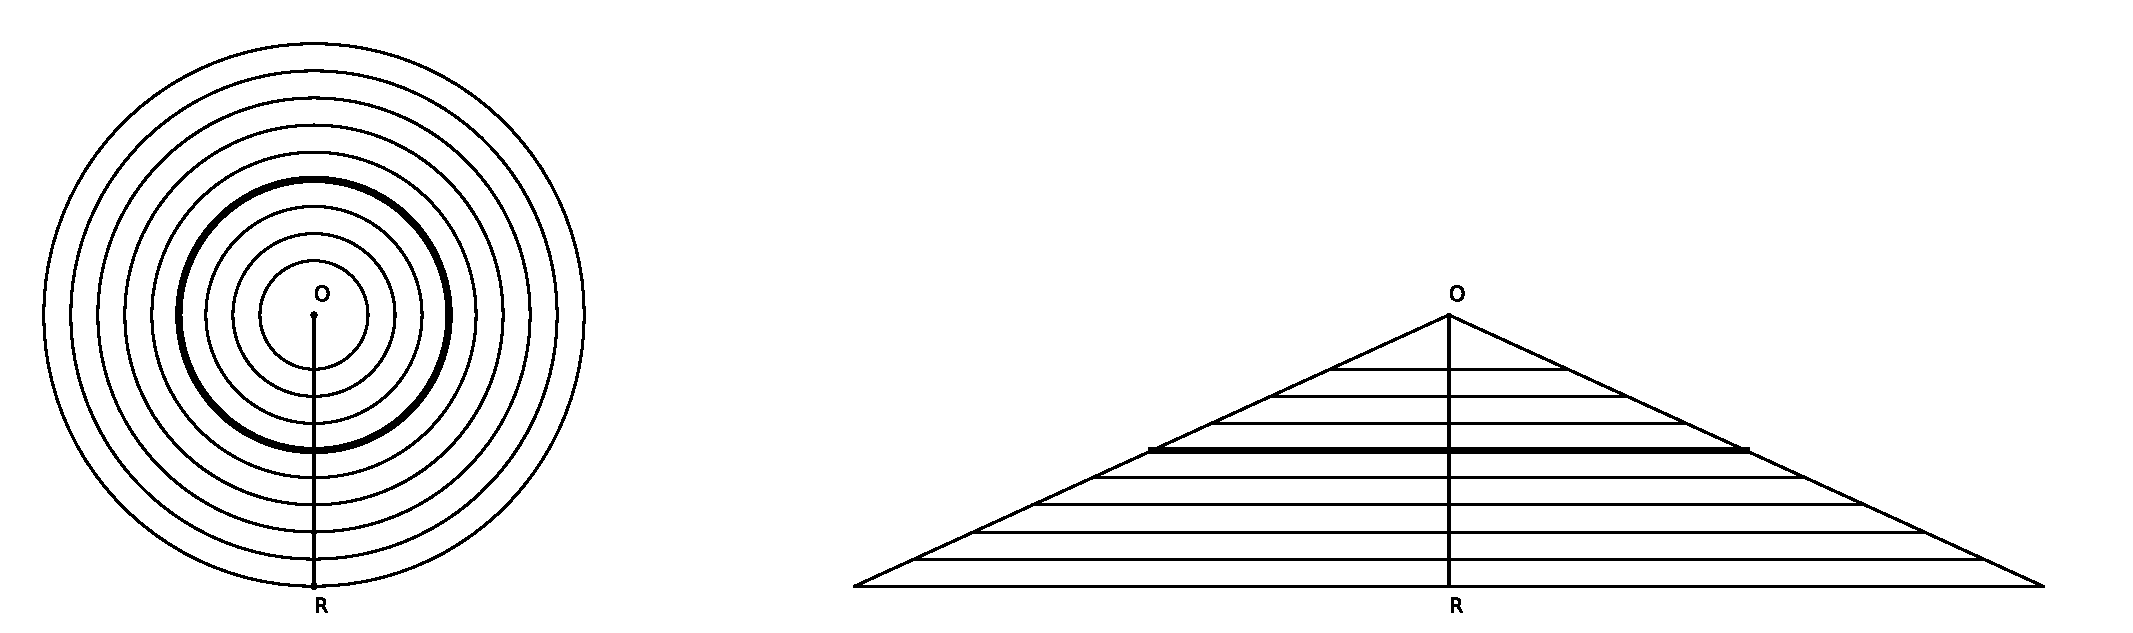
\includegraphics[scale=0.44]{images/archimed_1}
   \caption{Равносоставленность круга и треугольника.}
   \label{fig:archimed_1}
\end{figure}

Идею равносоставленности можно проиллюстрировать на следующем примере (см. рис. \ref{fig:archimed_1}).
Рассмотрим круг радиуса $R$ на плоскости.
Постараемся найти его площадь, зная что длина окружности есть произведение $2\pi$ на ее радиус.
Представим круг состоящим из неделимых объектов - концентрических окружностей с центром в центре круга.
Далее мысленно разрежем круг вдоль вертикального радиуса $OA$ и развернем каждую окружность в отрезок, сохранив ее длину и положение середины на нижнем радиусе $OR$.
В результате получится треугольник с основанием $2\pi R$ и высотой $R$.
По известной формуле, его площадь равна
$$
S = 2\pi R\cdot\frac{R}{2} = \pi R^2.
$$
Заметим, что исходный круг и полученный треугольник \textit{равносоставленны}: каждой внутренней окружности круга однозначно соответствует горизонтальный отрезок треугольника, причем той же самой длины.
Так что можно ожидать, что найденное значение равно искомой площади круга, что действительно верно.

К сожалению, принцип равносоставленности в такой интерпретации годится только для отдельных случаев и в целом неверен. 
Несложно придумать, как говорят в математике, \textit{контрпример} рассуждений подобного рода, приводящим к совершенно неверным результатам.
Интересно, что и сам Архимед не относился к этому методу как к строгому, вероятно зная, что он может привести к ошибкам.
Архимед использовал его скорее как способ угадать правильный ответ, который затем тщательно проверял.
И тем не менее, отношение к идее атомизма как конкретному математическому инструменту (пусть и не идеальному) позволило Евдоксу и Архимеду заложить основы современного интегрального исчисления, а вместе с ним и значительной части современной математики.

Идеи раннего атомизма, конечно же, довольно далеки от современного взгляда на вещи.
И тем не менее кажется удивительным то, насколько удалось продвинуться в своих размышлениях философам древности, не обладавшим серьезными измерительными приборами.
При должной фантазии в филосовских учениях восточной и древнегреческой философии вполне можно увидеть намеки на современное представление о микромире.
В буддизме, например, с древних времен фактически фигурировал вакуум как материальная среда, в которой мельчайшие частицы непрерывно возникают и исчезают. 
Сегодня подобный взгляд на вещи составляет основу квантовой теории поля, согласно которой так называемые \textit{виртуальные частицы} ведут себя схожим образом. 
Атомы по Демокриту участвовали в непрерывных случайных столкновениях друг с другом, порождая всевозможные движения объектов. 
Последнее весьма похоже на описание броуновского движения, если считать атомы Демокрита современными молекулами.

Философия атомизма была довольно популярна в древнем мире, но в итоге уступила философии Платона и Аристотеля, поддерживаемой набирающим силу христианством.
В период раннего Средневековья атомизм фактически находился под запретом господствующей религии и чуть не был утерян совсем.
Лишь в X веке к философии Демокрита стали постепенно и осторожно возвращаться.
Примечательно, что происходило это именно в христианских монастырях Англии и Ирландии.
Роль покровителя и популяризатора науки сыграл ученый и видный церковный и политический деятель Герберт Аврилакский.
Он с детства интересовался наукой и получил отличное по тем временам образование, проводя время за изучением достижений арабской и древнегреческой математики, астрономии и философии.
Вместе с этим он сделал блестящую карьеру в церкви, быстро став архиепископом, а затем и папой Сильвестром II.

Используя свое огромное влияние и сохранив приобретенную в юношестве тягу к знаниям, Герберт Аврилакский сыграл выдающуюся роль популяризации науки в целом и философии атомизма в частности.
Именно благодаря нему монастыри снова стали основными центрами просвещения своего времени.

Наконец, на рубеже средневековья и Нового времени об идеях Демокрита вновь заговорили открыто.
И опять, учение об атоме было воскрешено в XVII веке католическим священником. 
Пьер Гассенди был во многом выдающейся личностью своего времени. 
Аббат и профессор теологии в юношестве и профессор математики впоследствии, помимо богословия активно интересовался физикой, астрономией и математикой. 
Принятая Гассенди точка зрения на атомизм во многом повторяла учение Демокрита о пустом пространстве и существующих в нем неделимых элементах материи - атомах. 
Гассенди пошел дальше философов древности и впервые ввел в понятие \textit{молекулы} как соединения отдельных атомов. 
Согласно его точке зрения, все тела состоят из молекул, и именно молекулы определяют основные их свойства. 

Распространение атомизма в Средневековье во многом обязано отдельным выдающимся личностям, пытавшимся примирить его с гомподствующей религией.
Спорить с господствующей более 1000 лет точкой зрения могли только влиятельные религиозные и политические фигуры, но даже они довольно сильно рисковали.
Хотя нет прямых свидетельств жестокого преследования атомизма со стороны инквизиции, учение это было крайне непопулярно.
Его приверженцам зачастую приходилось приносить долгие официальные извинения.

Ценность этого исторического периода заключается не в конкретных достижениях, а самом факте того, что атомизм не был утерян совсем и продолжил свое развитие далее, в Новое время.


\section*{Новое время}

Идея молекулярного строения вещества была существенно развита в трудах выдающегося русского ученого М.В. Ломоносова в середине XVIII века.
Ломоносов пришел к заключению, что молекулы должны находиться в непрерывном движении и определять тепловое состояние тел.
Свою теорию ученый подтвердил математическими расчетами и рядом блестящих для того времени экспериментов.

.....




К началу XVIII века математический атомизм зарекомендовал себя как крайне эффективный и точный инструмент для самых разных вычислений в любых науках, где только возникали числа. 
Он стал прочным фундаментом для всей последующей математики как науки.
Практически весь аппарат математического анализа, развитого в трудах Ньютона, Лейбница, Кеплера, Лапласа, и многих других выдающихся ученых Нового времени, так или иначе можно считать развитием идей Архимеда и Евдокса.
Даже беглый обзор связанных с этим достижений в математике занял бы не одну главу и далеко увел бы нас от основного предмета книги - атома как физического объекта.
Здесь мы должны отвлечься от математического атомизма и вернуться к атомизму философскому, так как именно он в XVII-XVIII дал начало физике атома.


В Новое время изменились сами методы получения знаний о мире.
От чистого философствования они сместились к научному подходу, основанному на наблюдениях, экспериментах и вычислениях.
Именно это наконец позволило атомизму перейти из разряда чисто философской дисциплины в разряд прикладной науки. Выдвигались гипотезы и впервые появились методы их достоверной проверки.

Предстояло отчетливо понять различие между атомом и молекулой

.....



Идеи Нового времени дали второе рождение атомизму.
Это было время, когда начал активно использоваться совершенно новый подход к получению новых знаний - научный метод, основанный в меньшей степени на философии и в большей - на экспериментах, наблюдениях и вычислениях.
Хотя многие из высказанных верных предположений о строении материи все еще ждали своего строгого подтверждения, конкретные экспериментальные факты уже начали отделяться от чисто философских идей.

++++++++++==
Так был заложен прочный фундамент для физики микромира как строгой прикладной науки. 


Для настоящих же открытий нужен был совершенно новый подход, основанный в меньшей степени на философии и в большей - на научном методе. 
Необходимы были новые идеи, способные стать фундаментом для прикладной науки - физики микромира. 
Они появились только через 150 лет.

По словам Эйнштейна, ``воображение важнее знания, так как знание ограничено''.
В XX веке теории об атоме предстояло пережить... что даже вообрежени не всегда справлялось...


\section*{Время новой физики}

Серьезный прорыв был сделан в начале XIX века английским химиком Джоном Дальтоном, фактически возродившим атомизм. 
Дальтон сформулировал понятие атома, довольно близкое к современной точке зрения. 
Дальтон считал (и это верно), что атомы участвующих в химических превращениях веществ лишь перераспределяются, но не распадаются на части и не создаются. 
Таким образом, впервые возникла идея об атоме как \textit{химически неделимом} элементе мироздания, участвующем в любом превращении веществ в природе.


\section*{Строение атома}


\section*{Цепные реакции}


------------------------ IDEAS ------------------------ 





Атомизм как философское учение занимает особое место в философии древней Греции.
Воображение античных философов и их умение делать обобщения на основе наблюдаемых явлений природы позволило предвосхитить даже некоторые открытия недавнего прошлого.
Так философ Демокрит, один из основоположников древнегреческого атомизма, полагал, что вселенная состоит из \textit{пустоты} и \textit{атомов}. Атомы по Демокриту могут иметь разнообразную форму, в совокупности составляют отдельные объекты мира и участвуют в непрерывных столкновениях друг с другом, порождая всевозможные движения объектов.
Таким образом, Демокритом было фактически описано броуновское движение, если считать его атомы современными молекулами.

В древней индийской философии также в свое время родились и развивались концепции атомизма, причем, вероятно, даже раньше древнегреческих.
При всем многообразии конкурирующих религиозных школ и различии в своих учениях практически все они единогласно принимали концепцию атомизма в том или ином ее виде.
В буддизме идеи атомизма традиционно понимались гораздо шире, фактически основывая свое учение на понятии \textit{дхармы} как элементарной и неделимой сути объектов - центральном для всей буддийской философии.




XX век был поистине богатым научными открытиями в самых разных областях науки. Ученые как никогда приблизились к пониманию механики как микро, так и макро процессов окружающего мира. В биологии был обнаружен и описан основной строительный блок всего живого - молекула ДНК. Стремительно начала развиваться генная инженерия, находя приложения в самых разных отраслях человеческой деятельности. В физике были открыты общая и специальная теории относительности, квантовая механика. Выдающиеся достижения физиков и биологов активно освещались в прессе и практически сразу становились предметом жаркого обсуждения даже людьми, далекими от мира науки и в лучшем случае довольно приблизительно понимающими, о чем идет речь. 
Подобного, к сожалению, нельзя сказать об отношении к достижениям математики XX века - кроме самих математиков и, пожалуй, некоторых физиков, о них не знал практически никто. А они были поистине впечатляющими, вполне сравнимыми по потенциальной мощи с квантовой механикой или открытием ДНК. Стоит упомянуть хотя бы появление и активное использование компьютеров, необходимых для сложных расчетов тогда и распространенных повсеместно сейчас.

Отсутствие должного освещения открытий математики отчасти связано с самой спецификой данной науки. Лишь в редких случаях по-настоящему сложную математическую теорию можно объяснить широкому кругу людей-непрофессионалов. Чувство красоты математических рассуждений, доказательств и окончательных выводов необходимо упорно воспитывать в себе некоторое время, прежде чем появится понимание того, что стоит за длинными формулами и придет осознание того, как полученные выводы можно применить на практике.
Данная книга призвана восполнить этот пробел и рассказать, какую роль сыграли математики в знаменитом манхэттенском проекте, явившим миру всю мощь ядерной энергии. Я попытаюсь осветить мат. аппарат, который использовался при расчетах, связанных с конструированием атомной и водородных бомб, уделяя особое внимание методам, созданным именно в процессе работы над проектом “Манхэттен”.

Книга рассчитана на широкий круг читателей, интересующихся математикой и ее приложениями в ядерной физике. Книга будет интересна студентам и аспирантам физико-математических специальностей, а также просто интересующиеся тематикой атомной физики начала-середины XX века и применяемого там мат. аппарата. От читателей в большинстве случаем требуются лишь общие знания об основных понятиях математики - множествах и отображениях. Для понимания наиболее сложных моментов книги будет полезна специальная подготовка в рамках не ниже 2 курса физико-математических специальностей, общие знания по математическому анализу, теории вероятностей, дифференциальным уравнениям и функциональному анализу.






Формулу $E = mc^2$ как мантру может повторить практически любой современный человек.
Многие из нас так или иначе слышали о ней еще в детстве, не подозревая, что же она в действительности означает.
....


Попытки разобраться в сути какого-либо уже исследованном кем-то ранее явлении реального мира чем-то напоминают процесс очистки гипотетического фрукта с многослойной кожурой.
Первым и самым простым слоем являются личный опыт, мнения других людей и ``авторитетных'' источников о данном вопросе. 
На этом, собственно, можно и остановиться, сказав, что достаточно разобрались в вопросе.

Если полученные ответы нас не устраивают, не понятны, либо не полны и желание разобраться в сути явления не угасло, то придется перейти к следующему слою - предметной области явления, например, физике.
Необходимо хотя бы в общих чертах понять, что же именно происходит в интересующем нас явлении природы. 
Какие объекты в нем участвуют и по каким правилам взаимодействуют друг с другом. Какие моменты существенны, а какими можно пренебречь.
Продвинувшись в понимании физической сути процесса, мы 

Наконец, последний и традиционно самый трудный слой - математика явления.
Каждое явление природы имеет свой язык описания  ...  сложно .. вместо объектов - абстракции, вместо простых правил взаимодействия - сложные уравнения.



атомы - интуиция еще со времен древних греков, но дальше - перерыв почти на x000 лет связанный с тем, что увидеть объект своих измышлений уже не возможно.
прорыв - с появлением соответсвующих средств измерений, но тут ученых ждал очень большой сбрприз
до этого схема научных открытий в большинстве своем состояла в следующем - смотрели, измеряли, придумывали теорию основнную на уже известных аналогиях, потом совершенствовали приборы, и снова смотрели и придумывали анлогию и т.п.
в атомной физике известных аналогий не нашлось. Наблюдения зачастую в корне противоречили известным фактам о макромире. Любая попытка смотреть на макро-аналогии заканчивалась появлением множества противоречий теории с экспериментом и в конце концов полным провалом 


физика - ранее умение делать открытия зависело от того, насколько наблюдателен был ученый, насколько хорошо он умел проводить параллели между уже известными ялениями и только изучаемыми.
Движения огромных небесных тел описывалось исходя из аналогичных движений, которые можно было повторять в удобном масштабе в своей алборатории и т.п. [еще примеры]
Новая физика потребовала от ученых вообразить нечто не имевшее аналогов с ранее изученным в принципе. 
Это восхищало даже далеких от физики современников.
В математике такие штуки привыкли проворачивать довольно давно. 
Стефан Банах, один из создателей современной математики в ее [современном] виде, говорил "Хорошие математики видят аналогии, лучшие могут видеть аналигии между аналогиями". Сам он, безусловно, был одним из лучших.

 
слова "теория относительноси", "квантовая механик" носились в воздухе. Их можно было слышать  понимающих и истолковыва

----------------------------



https://ru.wikipedia.org/wiki/%D0%AD%D0%BB%D0%B5%D0%BA%D1%82%D1%80%D0%BE%D0%BD%D0%BD%D0%B0%D1%8F_%D0%BF%D0%BB%D0%BE%D1%82%D0%BD%D0%BE%D1%81%D1%82%D1%8C
{
В качестве модели состояния электрона в атоме, в квантовой механике принято представление об электронном облаке, плотность соответствующих участков которого пропорциональна вероятности нахождения там электрона.

Электронное облако часто изображают в виде граничной поверхности. При этом обозначение электронной области при помощи точек опускают. Пространство вокруг ядра, в котором наиболее вероятно пребывание электрона, называют атомной орбиталью (смысл которого вытекает из волнового уравнения Шрёдингера).

Применяются графические изображения распределения электронной плотности относительно ядра.

Кривая радиального распределения вероятности показывает, что электрон находится в тонком концентрическом шаровом слое радиуса r толщины dr вокруг ядра атома водорода[1].

Проекция максимума кривой соответствует боровскому радиусу alpha_0=0,53 A_with_circle.

Во многих случаях для решения уравнения Шрёдингера используют различные приближения. Вероятностную (статистическую) интерпретацию волновой функции разработал Макс Борн. В 1954 году М.Борн удостоен Нобелевской премии по физике с формулировкой «За фундаментальные исследования в области квантовой механики, особенно, за статистическую интерпретацию волновой функции.»
}

https://ru.wikipedia.org/wiki/%D0%A1%D1%82%D0%B0%D1%82%D0%B8%D1%81%D1%82%D0%B8%D1%87%D0%B5%D1%81%D0%BA%D0%B0%D1%8F_%D0%B8%D0%BD%D1%82%D0%B5%D1%80%D0%BF%D1%80%D0%B5%D1%82%D0%B0%D1%86%D0%B8%D1%8F_%D0%B2%D0%BE%D0%BB%D0%BD%D0%BE%D0%B2%D0%BE%D0%B9_%D1%84%D1%83%D0%BD%D0%BA%D1%86%D0%B8%D0%B8
{
М. Борн вспоминал:
Он (Шрёдингер) рассматривал электрон не как частицу, но как некоторое распределение плотности, которое давалось квадратом его волновой функции |ψ|².

Он считал, что следует полностью отказаться от идеи частиц и квантовых скачков, и никогда не сомневался в правильности этого убеждения. Я, напротив, имел возможность каждодневно убеждаться в плодотворности концепции частиц, наблюдая за блестящими опытами Франка по атомным и молекулярным столкновениям, и был убеждён, что частицы не могут быть упразднены. Следовало найти путь к объединению частиц и волн. Я видел связующее звено в идее вероятности…
}




